\subsection{Relay Internals}
\begin{figure}
\centering
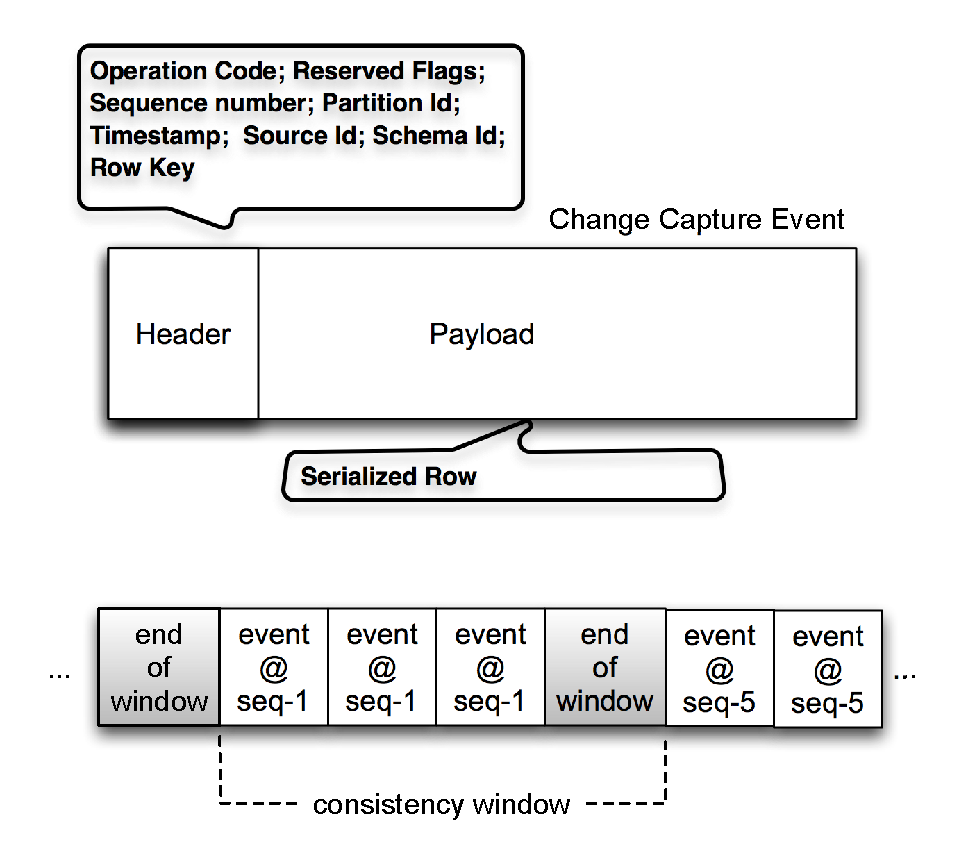
\epsfig{file=figures/change-capture-format.eps, width=3in}
\caption{Change Capture Window Format}
\label{fig:change-capture-window-format}
\end{figure}
As described earlier, the relay hosts a transient log store for low-latency serving of the change capture stream. When designing and implementing the relay, we tried to achieve the following goals:

\begin{itemize}

\item \emph{Low latency} and \emph{high throughput} for consumer pull requests
\item \emph{Low variance} for the latency of consumer pull requests
\item \emph{Scalability} to a large number of consumers
\item \emph{Multi-tenancy} of multiple change streams on the same relay

\end{itemize}

To achieve the above goals, we made some interesting design decisions. 

\begin{itemize}

\item \emph{Wire-format change buffer}: The change data is stored in memory using the on-wire serialization format in contiguous long-lived memory blocks outside the Java heap. This has two major benefits. First, it enables the use of high-throughput bulk-write operations to the network when serving pull requests. Second, it allows us to keep the change data in contiguous long-lived memory blocks outside the Java heap, thus, minimizing the GC pressure (low variance). 

\item \emph{Space-bound change buffer}: In addition to the above wire-format change buffer design, we wanted to support setting limits on how much space the buffer could use. This naturally led us to build it as a circular buffer with the changes pre-serialized and inlined. This supports very fast insert performance and also supports low latency range scans which are required for servicing the consumer pull requests. This also means we can easily estimate and control the memory utilization for the change data storage, thus, enabling multi-tenancy. 

\item \emph{Space-bound indexing}: Consumer pull requests perform range scans over the change data from the SCN of the last fetched change event. To allow efficient serving of such requests, we maintain an SCN index. The index is implemented as a skip-list on top of the change  buffer. As in the case of the change buffer, the index uses off-heap bounded memory for performance and multi-tenancy. This design also allows us to trade off some additional scan latency for reduced memory usage.

\item \emph{Fine-grained locking}: We use range-based locking to maximize read-write throughput for non-overlapping reads and writes. Writes acquire an exclusive lock on the region of the buffer to be over-written which is near the head of the buffer (the oldest events). Reads acquire a non-exclusive lock on a region from their starting read point to the tail of the buffer. Contention can occur only if a consumer is lagging behind and is trying to read older events. In practice, we hardly see any contention in our production workloads because readers and writers are pretty much in lock step most of the time. Further, read locks are generally short-lived (see below) so lagging readers cannot block the writer for a long time. If such readers further request events that have been  overwritten, they will be redirected to the Bootstrap Service and will not affect the relay performance.

\item \emph{Filtering}: We support server-side filtering by brute-force scanning the changes and streaming out only the events that match the subscriber's filter pattern. With the use of memory-mapped buffers, we avoid double-copying between user-space and file-system, and yet retain the ability to filter out data when we stream it out. The on-wire format of the change buffer incurs some CPU cost when applying the filter. In practice, we have found that the benefits of the chosen buffer implementation outweigh the costs as we are rarely bottle-necked on CPU utilization.

\item \emph{No consumer state}: As described in Section~\ref{sec:relay}, the relay does not maintain any per-consumer state. All information (e.g. the consumer checkpoint) needed to process a pull request is passed as part of the request. Most of the object allocation is associated with processing short-lived HTTP requests.

\item \emph{Short-lived pull requests}: All pull requests contain a limit on the size of the returned data. The subscription client requests only as much data as it can immediately buffer. The relay enforces aggressive timeouts when servicing pull requests. Because of this design decision and the off-heap storage of the change events and indexes, the relay has a trivial promotion rate to the old generation in the Java heap. This, coupled with the use of a CMS garbage collector, allows the relay to avoid long GC pauses and maintain low latency and low-variance response times.

\end{itemize}

Figure~\ref{fig:change-capture-window-format} shows the organization of a single consistency window in the change buffer. We decided to mark explicitly the end of consistency windows in the change stream. First, this allows the consumer to differentiate between the case of empty pull response because of no updates and the case of empty pull response because of no events matching the pull criteria. The former will return no changes; the latter will return the markers for the scanned windows. Thus, the subscription client can avoid processing the same change events on subsequent pulls. Second, end-of-window markers allow us to pass additional meta data (like checksums) about the windows.

\begin{figure}
\centering
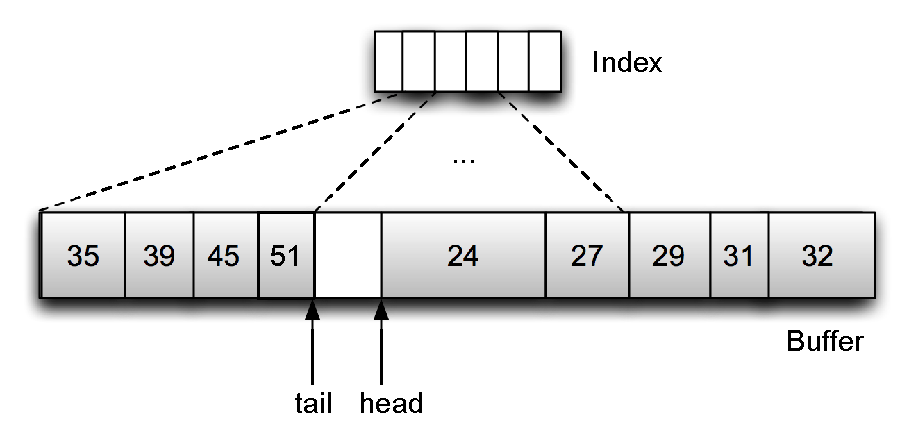
\epsfig{file=figures/relay-data-structures.eps, width=3.2in}
\caption{Buffer and Index Data Structures}
\label{fig:buffer-index}
\end{figure}
Figure~\ref{fig:buffer-index} summarizes the data structures used to implement the log store. 


%\begin{algorithm}
%\label{alg:stream-call}{stream}{($checkpoint$, $sources$, $filters$, $maxBytes$, $channel$)}
%\caption{Algorithm for servicing consumer pull requests}
%\begin{algorithmic}
%\STATE Consult index to determine the start of the scan
%\STATE Acquire read range lock from $scanOffset$ to $tail$
%\FOR{$event$ in $range$($scanOffset$, $tail$)}
%\IF{the $event$ is an end-of-window marker or it matches the $filters$ and we have not exceeded $maxBytes$}
%\STATE write $event$ to the $channel$
%\ENDIF
%\ENDFOR
%\STATE write $endOfStreamMarker$ to the $channel$
%\end{algorithmic}
%\end{algorithm} 

%The pseudo-code for servicing the consumer pull request is documented at Algorithm~\ref{alg:stream-call}. The primary input parameters into this call are the consumer's checkpoint, the list of tables they are interested in and any subscription filters that they want to apply additionally on the changes. The call first determines the scan offset to begin the scan, and then acquires a read range lock from the offset to the tail of the buffer. It then iterates through the buffer streaming out any events that match the filter. The stopping condition is either reaching the end of the buffer or hitting the maximum size limit set by the consumer. 

The consumer pull request is serviced through the \emph{getSince} method in the Relay. The primary input parameters into this call are the consumer's checkpoint, the list of tables they are interested in and any subscription filters that they want to apply additionally on the changes. We first determine the scan offset to begin the scan by consulting the index. We then acquire a read range lock from the scan offset to the tail of the buffer. We then iterate through the buffer streaming out any events that match the filter. The stopping condition is either reaching the tail or hitting the maximum size limit set by the consumer. 



